% Implementation chapter continued
\section{RabbitMQ as a Central Message Bus}\label{internals}
RabbitMQ is a sophisticated version of messaging queue and its application in this thesis makes the
project unique. Each block(subsystem) of mercator design consists of one or more pair of consumer and producer inside RabbitMQ that subscribes and publishes events, shown in figure \ref{fig:rmq}.
\begin{figure}[h!]
  \centering
  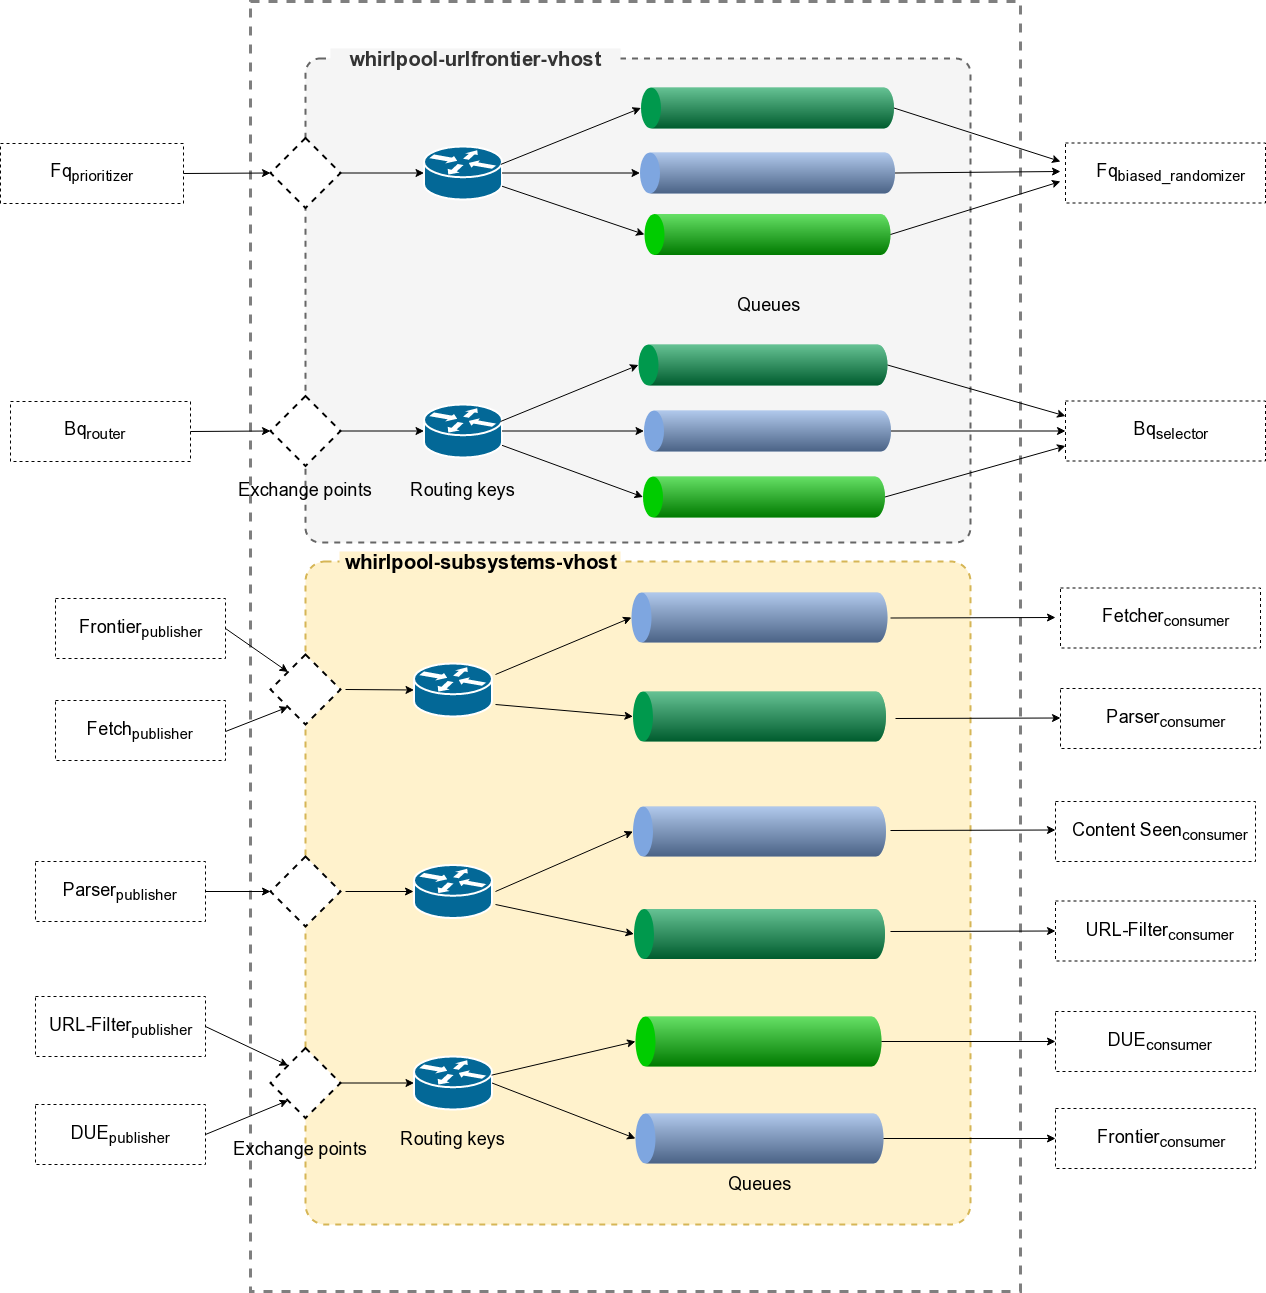
\includegraphics[width=20cm,height=15cm,keepaspectratio]{../media/crawler/rmq-broker.png}
  \caption{Message Distribution using RabbitMQ Direct Exchange}
  \label{fig:rmq}
\end{figure}

\noindent
Direct worker queue\cite{asyncmsg} is one of the three well known message routing methods used to communicate with the
queues. In this case, the consumer on one end has to know the name of the queue while the producer has to know the exchange name only and not the queue to deliver event message to the right consumer subscribed to it.
RabbitMQ's internal routing decouples (also promotes open/close principle) producer from consumer, both physically and logically. This manifestation reminds us of service-oriented architecture style(SOA). Each
pair is a autonomous service, fairly generic, focusing on one particular problem, wired together to build complex chain of producers and consumers thus completing the crawler design.
\\
\\
\noindent
RabbitMQ is used to decide which blocks of the mercator should communicate with each other and how the
messages should flow through the queues. The Queues are logically grouped into two different virtual
host(vhost) - the frontier vhost and the subsystems vhost. The idea behind vhost in RabbitMQ is similar
to vhost in apache, however, the difference is vhost in RabbitMQ are created using HTTP APIs whereas
in apache they are specified in conf file. Each block authenticates to its designated vhost which has
appropriate resource permissions preset. The queues for URL frontier solely lives in frontier vhost
whereas the fetcher, parser, seentest, filter, and the due queues reside in subsystems vhost, see figure
\ref{fig:rmq}. Interconnection between the vhost exist at the vhost generic consumer-producer processes.
\\
\\
\noindent
Consumer threads using Frontier queues use the pull model because consumer pulls messages from the queue.
On the other hand, push model is used for consumers under subsystems vhost. It is model in which the
consumer runs constantly in an infinite loop, getting a persistent connection to the message broker.

\pagebreak

\section{Shared Services with Docker}
\begin{figure}[h!]
  \centering
  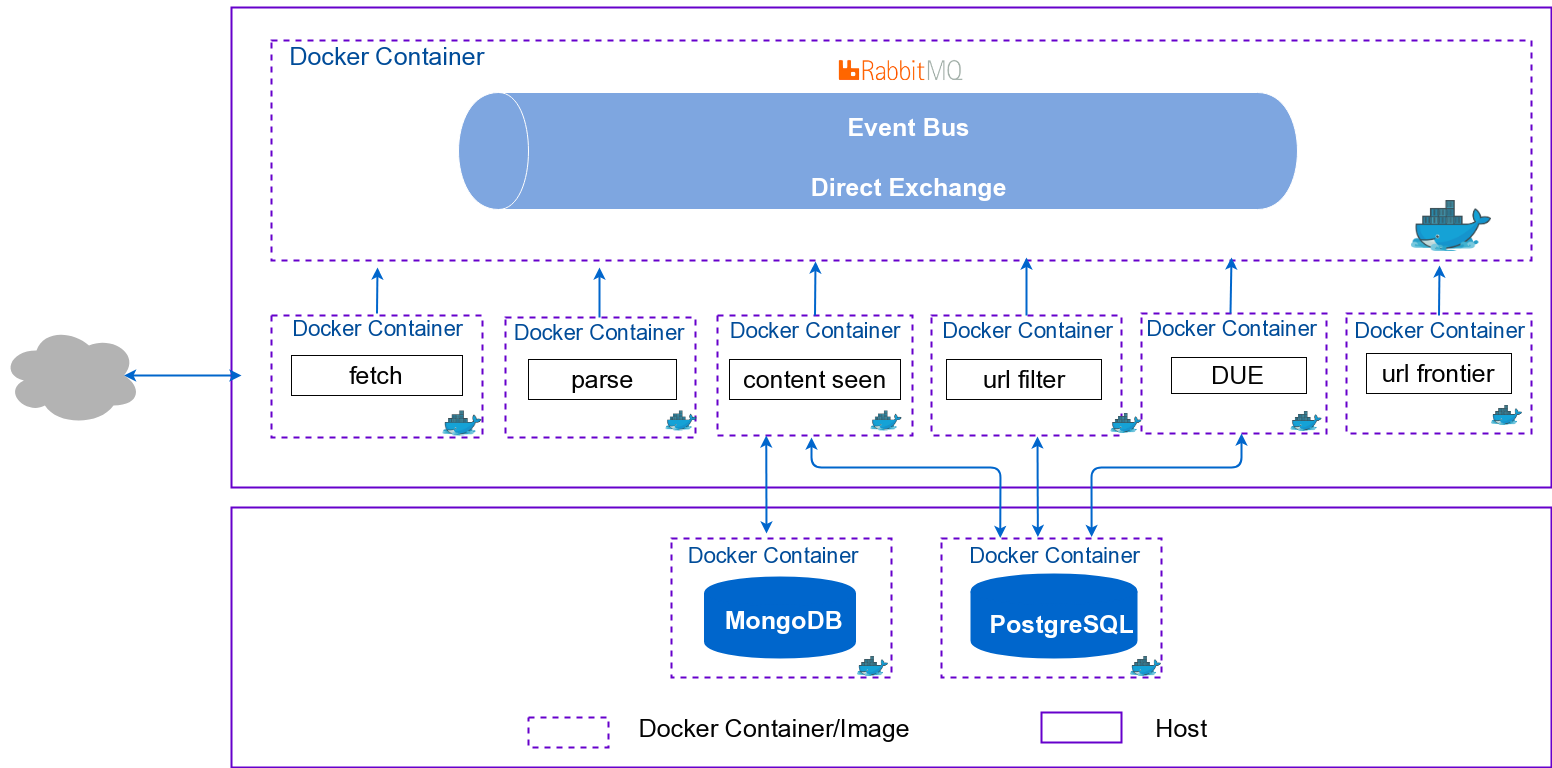
\includegraphics[width=18cm,height=10cm,keepaspectratio]{../media/crawler/multi-container-deploy.png}
  \caption{Single-node Whirlpool Subsystem Isolation using Docker}
  \label{fig:multicontainer}
\end{figure}

\noindent
This is the production and development state of whirlpool containers that is deployed in the AWS cloud.
Afterall, this is a whole point of using containerization. All it takes is a orchestration file that
reads production level configuration when deploying on AWS. One exception here in figure
\ref{fig:multicontainer} is that in production environment, postgresql database is a AWS RDS instance and
during local development postgresql is self contained docker container. A clear distinction is made to
distinguish service running directly on provisioned machine or in a container. Each solid box is a
separate machine and dashed box is a container on that machine.
\\
\\
\noindent
The state of mongodb, postgres is separated from the state of each crawler node and shared with each
running instance of crawler. The state of RabbitMQ is local to machine its running on. This becomes a
stateless, shared nothing architecture. Each message flowing through the queue is independent of the other.
Load sharing among other running instance of crawler is not based on hostname but instead uses
consistent hashing, see section \ref{distcrawl} to understand the benefits of it. 
\\
\\
\noindent
The fetch subsystem has the job to visit the html page and the result of it can have many different
outcomes. Blocking messages in queue until the current url is complete can leave the consumer stranded and
messages piling up in the fetch queue. Depending on the language runtime used, fetch's consumer script
should either be multi-threaded or process urls in asynchronous fashion. The later approach is adopted
using nodejs. Handling of politeness and coordinating priority of urls to crawl is a multi-threaded jar
executable written in java.
\pagebreak

\section{Developing code with Docker}\label{devdocker}
At the foundation of any dockerized program, \texttt{dockerfile} is a place to package source code. The biggest advantage of using containerization as discussed in section \ref{dockerintro}, is to get same program behavior under development and production environments, making deployment process easier. At first, a developer will use \texttt{dockerfile} for developmental use. This approach, however, is time-consuming, slows speedy development as docker engine takes a while to build \& re-run on every change. Whats even worse is that the size of development image gets bigger on each build as dependencies are added/removed, updates to the base images are installed. This actions aren't required when developing code. 
\\
\\
The best practice when developing code with docker is to use \texttt{docker-compose.yml} to define the environment at different layers. The version 2 of compose file allows to extend and reuse existing layers. Version 2 is more developer friendly while
version 3 is geared towards production use. As you can in below image under
\texttt{services} directive - install and quick-up project services extend base
project.

\inputminted[
fontfamily=tt,
baselinestretch=1.2,
fontsize=\footnotesize,
linenos,
breaklines,
numbersep=5pt,
tabsize=2,
firstline=1,
lastline=30,
frame=single]{yaml}{../../whirlpool/crawler/whirlpool-fetch/docker-compose.build.yml}

\pagebreak

\inputminted[
fontfamily=tt,
baselinestretch=1.2,
fontsize=\footnotesize,
linenos,
breaklines,
numbersep=5pt,
tabsize=2,
firstline=31,
lastline=34,
frame=single]{yaml}{../../whirlpool/crawler/whirlpool-fetch/docker-compose.build.yml}

\noindent
The environment defines external \texttt{network} sharing it with containers defined outside and inside the compose file. This is specific to development setup where 
one component is actively getting developed while others are in ready state. Similarly, the external \texttt{volume} persist javascript(in this example) dependencies outside the container, thus allowing sharing among other containers such as install and quick-up services.

\inputminted[
fontfamily=tt,
baselinestretch=1.2,
fontsize=\footnotesize,
linenos,
numbersep=5pt,
tabsize=2,
firstline=1,
lastline=14,
frame=single]{make}{../../whirlpool/crawler/whirlpool-fetch/Makefile}

\noindent
The use of \texttt{Makefile} makes docker commands easier to remember when typing on the command line. Note that the same commands can also be integrated into IDE of choice.

\begin{lstlisting}[language=bash]
  $ make install
\end{lstlisting}

\noindent
Trying the above command for the very first time will establish network, pull node image only once and install dependencies to the specified external volume. This is for the project defined in \texttt{docker-compose.build.yml}.

\begin{lstlisting}[language=bash]
  $ make quick-up
\end{lstlisting}

\noindent
Once the packages are installed, and after having made some changes to the code. The
program is launched using the above command. It runs inside the container with
installed packages shared by base servive. The flow is pretty fast as the install
and run operations are isolated and there is no time wasted in building and
packaging on every iteration of code change. This is very much ideal and
correct way to use docker while writing code.

\begin{lstlisting}[language=bash]
  $ make prod-build && make tag-prod && make push-prod
\end{lstlisting}
\noindent
This command clubs 3 commands - packages code for running on production machine, labels the image and pushes it to a central docker repository.

\pagebreak

\section{Policy of assigning priorities \& picking queues}
\begin{figure}[h!]
  \centering
  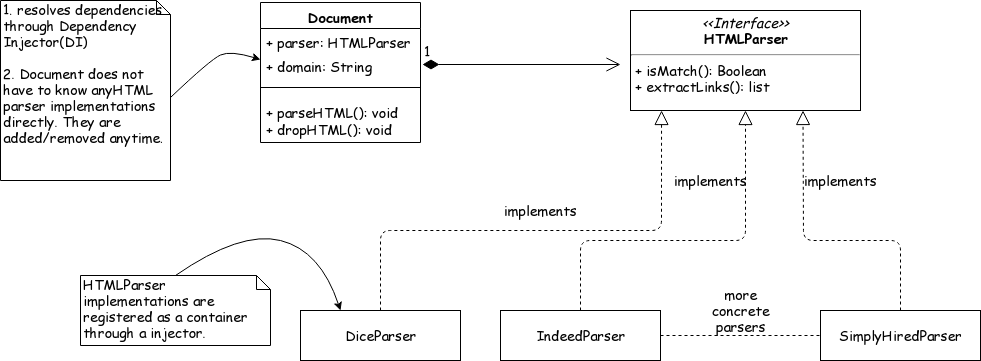
\includegraphics[width=15cm,height=12cm,keepaspectratio]{../media/crawler/docparsers.png}
  \caption{Whirlpool Parser subsystem using Dependency Injection}
  \label{fig:htmlparser}
\end{figure}

\noindent
Figure \ref{fig:htmlparser} is a class diagram for parser subsystem. Its uses the Dependency Injection
design pattern discussed in background chapter, section \ref{softdesign}. DiceParser, IndeedParser, etc are
concrete implementations of HTMLParser class. Each represents a parser for set of seeds shown in figure
\ref{fig:missionchar}. Each of which is a knowledgeable to understand given page relevance followed by assigning single digit numeric weight to extracted urls from the given page. The URLs flow through various message queues until it lands in frontier queues where they are organized into different priority levels. 
\\
\\
\noindent
The Document class is highly decoupled from those array of concrete classes. During runtime, the
concrete classes are loaded by the dependency inject. Upon receiving message from the queue, it invokes
\textit{isMatch()}, \textit{extractLinks()} on one of those concrete classes based on the metadata in the
message.

\pagebreak



